\documentclass[12pt,a4paper]{article}
\usepackage[utf8]{vietnam}
\usepackage{amsmath,amssymb}
\usepackage{tabularx}
\usepackage{tikz}
\usepackage{xcolor}
\usepackage[top=0.6cm, bottom=0.6cm, left=0.6cm, right=0.6cm]{geometry}
\usepackage[dethi]{ex_test}

\SAOPTN{widthSA=2.6,heightSA=0.62}
\setlength{\parskip}{0pt}

% Dong ke cham mo chuan viet tay
\newcommand{\dongke}[1]{%
  \begingroup%
  \setlength{\parskip}{0pt}%
  \baselineskip=18.5pt%
  \vspace{1.0mm}%
  \foreach \i in {1,...,#1}{%
    \noindent{\color{gray!60}\dotfill}\par%
  }%
  \vspace{0.6mm}%
  \endgroup%
}

% Khu vuc bai lam chia 2 cot co vach ngan mo o giua
\newcommand{\dongkeHaiCot}[1]{%
  \par\vspace{0.5mm}%
  \noindent%
  \begin{minipage}[t]{0.485\linewidth}%
    \dongke{#1}%
  \end{minipage}%
  \hfill%
  {\color{gray!60}\vrule}%
  \hfill%
  \begin{minipage}[t]{0.485\linewidth}%
    \dongke{#1}%
  \end{minipage}%
}

% Dinh nghia o bai tap tu luan trong bang
\newcommand{\oBaiTap}[3][5]{%
  \vspace{1.0mm}%
  \noindent\textbf{#2} #3\par%
  \dongke{#1}%
}

\begin{document}
\pagestyle{empty}
% =============================================================================
% ========================= TOAN 8 TUAN 10 BUOI 02 - MA DE 101 =================
% ========================= TRANG 1/2 ==========================================
% =============================================================================
\noindent
\begin{tabularx}{\linewidth}{|X|c|}
\hline
\textbf{PHIẾU KIỂM TRA ĐỊNH KỲ TOÁN 8 - TUẦN 10 - BUỔI 2} & \textbf{Mã đề: 101 - Trang 1/2} \\
\hline
\end{tabularx}

\vspace{1.2mm}

\noindent
\begin{tabularx}{\linewidth}{|p{3.2cm}|X|}
\hline
\centering\textbf{ĐIỂM SỐ} & \centering\textbf{LỜI NHẬN XÉT CỦA THẦY CÔ} \tabularnewline
\hline
\rule{0pt}{1.8cm} & \tabularnewline
\hline
\end{tabularx}

\vspace{1.4mm}
\noindent\textbf{Câu 1 (0,25 điểm).} Cho $\Delta ABC, M \in AB, N \in AC$ có $\dfrac{AM}{MB} = \dfrac{AN}{NC}$. Khi đó $MN \dots BC$: \shortans{\parallel}\par\vspace{2.0mm}
\noindent\textbf{Câu 2 (0,25 điểm).} $\Delta ABC, MN \parallel BC$. Biết $AM=2, AB=6, BC=9\text{ cm}$. Độ dài $MN$ là: \shortans{3\text{ cm}}\par\vspace{2.0mm}
\noindent\textbf{Câu 3 (0,25 điểm).} Cho $\Delta ABC$ có $DE \parallel BC$. Biết $AD=3, DB=2$. Tỉ số $\dfrac{DE}{BC}$ bằng: \shortans{\frac{3}{5}}\par\vspace{2.0mm}
\noindent\textbf{Câu 4 (0,25 điểm).} Phân tích đa thức $3x^2 - 6x$ thành nhân tử được: \shortans{3x(x - 2)}\par\vspace{2.0mm}
\noindent\textbf{Câu 5 (0,25 điểm).} Phân tích đa thức $x^2 - 25$ thành nhân tử được: \shortans{(x - 5)(x + 5)}\par\vspace{2.0mm}
\noindent\textbf{Câu 6 (0,25 điểm).} Thu gọn biểu thức $x^2 + 6x + 9$ thành bình phương được: \shortans{(x + 3)^2}\par\vspace{2.0mm}
\noindent\textbf{Câu 7 (0,25 điểm).} Bậc của đa thức $P = 4x^3 y^2 - 5x^2 y^3 + 2xy - 1$ là: \shortans{5}\par\vspace{2.0mm}
\noindent\textbf{Câu 8 (0,25 điểm).} Kết quả của phép chia $(18x^5 y^4) : (6x^3 y^2)$ là: \shortans{3x^2 y^2}\par\vspace{2.0mm}
\noindent\textbf{Câu 9 (0,25 điểm).} Định lí Thalès đảo dùng để chứng minh hai đường thẳng: \shortans{\text{song song}}\par\vspace{2.0mm}
\noindent\textbf{Câu 10 (0,25 điểm).} Bờ sông có $MN \parallel AB$: $OM=4, MA=8, MN=6\text{ m}$. Tính $AB$: \shortans{18\text{ m}}\par\vspace{2.0mm}
\vspace{0.2mm}
\noindent\textbf{Câu 11 (3,0 điểm). Thực hiện phép tính và phân tích đa thức thành nhân tử:}
\vspace{0.8mm}

\noindent
\begin{tabularx}{\linewidth}{|X|X|}
\hline
\oBaiTap[5]{a) (0,5 điểm)}{$3x(2x^2 - 5x + 3)$} & 
\oBaiTap[5]{b) (0,5 điểm)}{$(x - 1)(x + 4) - (x^2 - 4)$} \\
\hline
\oBaiTap[5]{c) (0,5 điểm)}{$(2x - 3)^2 + (2x + 3)^2$} & 
\oBaiTap[5]{d) (0,5 điểm)}{Phân tích nhân tử: $xy - 3x + 2y - 6$} \\
\hline
\oBaiTap[5]{e) (0,5 điểm)}{Phân tích nhân tử: $x^2 - y^2 + 4x + 4$} & 
\oBaiTap[5]{f) (0,5 điểm)}{Phân tích nhân tử: $x^2 - 7x + 12$} \\
\hline
\end{tabularx}

\newpage
% =============================================================================
% ========================= TOAN 8 TUAN 10 BUOI 02 - MA DE 101 =================
% ========================= TRANG 2/2 ==========================================
% =============================================================================
\noindent
\begin{tabularx}{\linewidth}{|X|c|}
\hline
\textbf{TOÁN 8 - TUẦN 10 - BUỔI 2} & \textbf{Mã đề: 101 - Trang 2/2} \\
\hline
\end{tabularx}

\vspace{1.4mm}

\noindent\textbf{Câu 12 (2,0 điểm). Tìm số thực $x$, biết:}
\vspace{0.8mm}

\noindent
\begin{tabularx}{\linewidth}{|X|X|}
\hline
\oBaiTap[5]{a) (0,5 điểm)}{$2x(x - 4) - 2x^2 = 16$} & 
\oBaiTap[5]{b) (0,5 điểm)}{$x(x - 3) - 5(x - 3) = 0$} \\
\hline
\oBaiTap[5]{c) (0,5 điểm)}{$(x - 2)^2 - 16 = 0$} & 
\oBaiTap[5]{d) (0,5 điểm)}{$(2x + 3)^2 = 49$} \\
\hline
\end{tabularx}

\vspace{1.4mm}

\noindent
\begin{tabularx}{\linewidth}{|X|}
\hline
\vspace{0.5mm}
\begin{minipage}[t]{0.68\linewidth}
\vspace{0pt}
\textbf{Câu 13 (2,0 điểm).} Cho tam giác $ABC$. Trên cạnh $AB$ lấy điểm $M$, trên cạnh $AC$ lấy điểm $N$. Cho biết $AM = 4\text{ cm}, MB = 6\text{ cm}, AN = 6\text{ cm}, NC = 9\text{ cm}$ và $BC = 15\text{ cm}$.\par\vspace{0.4mm}
\textbf{a)} \textbf{(1,0 điểm)} Chứng minh rằng $MN \parallel BC$.\par\vspace{0.4mm}
\textbf{b)} \textbf{(1,0 điểm)} Tính độ dài đoạn thẳng $MN$.
\end{minipage}\hfill
\begin{minipage}[t]{0.30\linewidth}
\vspace{0pt}\centering
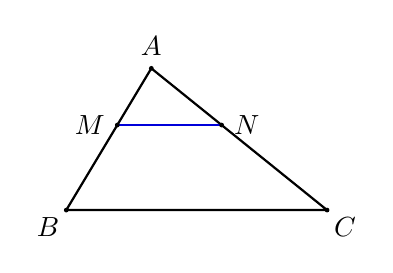
\begin{tikzpicture}[scale=0.72, >=stealth, line join=round, line cap=round]
  \coordinate (B) at (0, 0);
  \coordinate (C) at (4.6, 0);
  \coordinate (A) at (1.5, 2.5);
  \coordinate (M) at (0.9, 1.5);
  \coordinate (N) at (2.74, 1.5);
  \draw[thick] (A) -- (B) -- (C) -- cycle;
  \draw[thick, blue!85!black] (M) -- (N);
  \fill (A) circle (1.2pt) node[above=1pt] {$A$};
  \fill (B) circle (1.2pt) node[below left=-1pt] {$B$};
  \fill (C) circle (1.2pt) node[below right=-1pt] {$C$};
  \fill (M) circle (1.2pt) node[left=1pt] {$M$};
  \fill (N) circle (1.2pt) node[right=1pt] {$N$};
\end{tikzpicture}
\end{minipage}\par
\vspace{0.4mm}
\noindent\textit{Bài giải:}\dongkeHaiCot{11}
\\ \hline
\end{tabularx}

\vspace{1.4mm}

\noindent
\begin{tabularx}{\linewidth}{|X|}
\hline
\vspace{0.5mm}
\textbf{Câu 14 (0,5 điểm).} Tìm giá trị lớn nhất của biểu thức $P = -x^2 + 6x + 2020$.\par
\vspace{0.4mm}
\noindent\textit{Bài giải:}\dongkeHaiCot{7}
\\ \hline
\end{tabularx}

\newpage
% =============================================================================
% ========================= TOAN 8 TUAN 10 BUOI 02 - MA DE 102 =================
% ========================= TRANG 1/2 ==========================================
% =============================================================================
\noindent
\begin{tabularx}{\linewidth}{|X|c|}
\hline
\textbf{PHIẾU KIỂM TRA ĐỊNH KỲ TOÁN 8 - TUẦN 10 - BUỔI 2} & \textbf{Mã đề: 102 - Trang 1/2} \\
\hline
\end{tabularx}

\vspace{1.2mm}

\noindent
\begin{tabularx}{\linewidth}{|p{3.2cm}|X|}
\hline
\centering\textbf{ĐIỂM SỐ} & \centering\textbf{LỜI NHẬN XÉT CỦA THẦY CÔ} \tabularnewline
\hline
\rule{0pt}{1.8cm} & \tabularnewline
\hline
\end{tabularx}

\vspace{1.4mm}
\noindent\textbf{Câu 1 (0,25 điểm).} Cho $\Delta ABC, M \in AB, N \in AC$ có $\dfrac{AM}{AB} = \dfrac{AN}{AC}$. Khi đó $MN \dots BC$: \shortans{\parallel}\par\vspace{2.0mm}
\noindent\textbf{Câu 2 (0,25 điểm).} $\Delta ABC, MN \parallel BC$. Biết $AM=3, AB=9, BC=12\text{ cm}$. Độ dài $MN$ là: \shortans{4\text{ cm}}\par\vspace{2.0mm}
\noindent\textbf{Câu 3 (0,25 điểm).} Cho $\Delta ABC$ có $DE \parallel BC$. Biết $AD=4, DB=3$. Tỉ số $\dfrac{DE}{BC}$ bằng: \shortans{\frac{4}{7}}\par\vspace{2.0mm}
\noindent\textbf{Câu 4 (0,25 điểm).} Phân tích đa thức $4x^2 - 8x$ thành nhân tử được: \shortans{4x(x - 2)}\par\vspace{2.0mm}
\noindent\textbf{Câu 5 (0,25 điểm).} Phân tích đa thức $x^2 - 36$ thành nhân tử được: \shortans{(x - 6)(x + 6)}\par\vspace{2.0mm}
\noindent\textbf{Câu 6 (0,25 điểm).} Thu gọn biểu thức $x^2 - 8x + 16$ thành bình phương được: \shortans{(x - 4)^2}\par\vspace{2.0mm}
\noindent\textbf{Câu 7 (0,25 điểm).} Bậc của đa thức $Q = 6x^4 y - 2x^2 y^3 + 3x^3 y^2 - 9$ là: \shortans{5}\par\vspace{2.0mm}
\noindent\textbf{Câu 8 (0,25 điểm).} Kết quả của phép chia $(24x^6 y^5) : (8x^4 y^3)$ là: \shortans{3x^2 y^2}\par\vspace{2.0mm}
\noindent\textbf{Câu 9 (0,25 điểm).} Định lí Thalès thuận dùng để tính đại lượng nào của hình: \shortans{\text{độ dài cạnh}}\par\vspace{2.0mm}
\noindent\textbf{Câu 10 (0,25 điểm).} Bờ sông có $MN \parallel AB$: $OM=5, MA=10, MN=7\text{ m}$. Tính $AB$: \shortans{21\text{ m}}\par\vspace{2.0mm}
\vspace{0.2mm}
\noindent\textbf{Câu 11 (3,0 điểm). Thực hiện phép tính và phân tích đa thức thành nhân tử:}
\vspace{0.8mm}

\noindent
\begin{tabularx}{\linewidth}{|X|X|}
\hline
\oBaiTap[5]{a) (0,5 điểm)}{$4x(2x^2 - 3x + 4)$} & 
\oBaiTap[5]{b) (0,5 điểm)}{$(x - 2)(x + 5) - (x^2 - 10)$} \\
\hline
\oBaiTap[5]{c) (0,5 điểm)}{$(3x - 2)^2 + (3x + 2)^2$} & 
\oBaiTap[5]{d) (0,5 điểm)}{Phân tích nhân tử: $xy - 4x + 3y - 12$} \\
\hline
\oBaiTap[5]{e) (0,5 điểm)}{Phân tích nhân tử: $x^2 - y^2 + 6x + 9$} & 
\oBaiTap[5]{f) (0,5 điểm)}{Phân tích nhân tử: $x^2 - 8x + 15$} \\
\hline
\end{tabularx}

\newpage
% =============================================================================
% ========================= TOAN 8 TUAN 10 BUOI 02 - MA DE 102 =================
% ========================= TRANG 2/2 ==========================================
% =============================================================================
\noindent
\begin{tabularx}{\linewidth}{|X|c|}
\hline
\textbf{TOÁN 8 - TUẦN 10 - BUỔI 2} & \textbf{Mã đề: 102 - Trang 2/2} \\
\hline
\end{tabularx}

\vspace{1.4mm}

\noindent\textbf{Câu 12 (2,0 điểm). Tìm số thực $x$, biết:}
\vspace{0.8mm}

\noindent
\begin{tabularx}{\linewidth}{|X|X|}
\hline
\oBaiTap[5]{a) (0,5 điểm)}{$3x(x - 3) - 3x^2 = 18$} & 
\oBaiTap[5]{b) (0,5 điểm)}{$x(x - 4) - 6(x - 4) = 0$} \\
\hline
\oBaiTap[5]{c) (0,5 điểm)}{$(x - 3)^2 - 25 = 0$} & 
\oBaiTap[5]{d) (0,5 điểm)}{$(2x - 1)^2 = 49$} \\
\hline
\end{tabularx}

\vspace{1.4mm}

\noindent
\begin{tabularx}{\linewidth}{|X|}
\hline
\vspace{0.5mm}
\begin{minipage}[t]{0.68\linewidth}
\vspace{0pt}
\textbf{Câu 13 (2,0 điểm).} Cho tam giác $ABC$. Trên cạnh $AB$ lấy điểm $M$, trên cạnh $AC$ lấy điểm $N$. Cho biết $AM = 6\text{ cm}, MB = 9\text{ cm}, AN = 8\text{ cm}, NC = 12\text{ cm}$ và $BC = 20\text{ cm}$.\par\vspace{0.4mm}
\textbf{a)} \textbf{(1,0 điểm)} Chứng minh rằng $MN \parallel BC$.\par\vspace{0.4mm}
\textbf{b)} \textbf{(1,0 điểm)} Tính độ dài đoạn thẳng $MN$.
\end{minipage}\hfill
\begin{minipage}[t]{0.30\linewidth}
\vspace{0pt}\centering
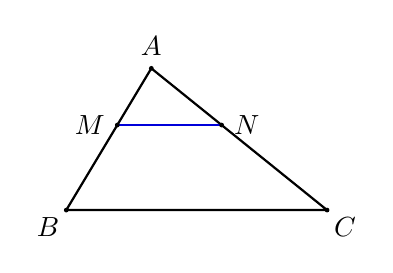
\begin{tikzpicture}[scale=0.72, >=stealth, line join=round, line cap=round]
  \coordinate (B) at (0, 0);
  \coordinate (C) at (4.6, 0);
  \coordinate (A) at (1.5, 2.5);
  \coordinate (M) at (0.9, 1.5);
  \coordinate (N) at (2.74, 1.5);
  \draw[thick] (A) -- (B) -- (C) -- cycle;
  \draw[thick, blue!85!black] (M) -- (N);
  \fill (A) circle (1.2pt) node[above=1pt] {$A$};
  \fill (B) circle (1.2pt) node[below left=-1pt] {$B$};
  \fill (C) circle (1.2pt) node[below right=-1pt] {$C$};
  \fill (M) circle (1.2pt) node[left=1pt] {$M$};
  \fill (N) circle (1.2pt) node[right=1pt] {$N$};
\end{tikzpicture}
\end{minipage}\par
\vspace{0.4mm}
\noindent\textit{Bài giải:}\dongkeHaiCot{11}
\\ \hline
\end{tabularx}

\vspace{1.4mm}

\noindent
\begin{tabularx}{\linewidth}{|X|}
\hline
\vspace{0.5mm}
\textbf{Câu 14 (0,5 điểm).} Tìm giá trị lớn nhất của biểu thức $Q = -x^2 + 8x + 2010$.\par
\vspace{0.4mm}
\noindent\textit{Bài giải:}\dongkeHaiCot{7}
\\ \hline
\end{tabularx}

\newpage
% =============================================================================
% ========================= TOAN 8 TUAN 10 BUOI 02 - MA DE 103 =================
% ========================= TRANG 1/2 ==========================================
% =============================================================================
\noindent
\begin{tabularx}{\linewidth}{|X|c|}
\hline
\textbf{PHIẾU KIỂM TRA ĐỊNH KỲ TOÁN 8 - TUẦN 10 - BUỔI 2} & \textbf{Mã đề: 103 - Trang 1/2} \\
\hline
\end{tabularx}

\vspace{1.2mm}

\noindent
\begin{tabularx}{\linewidth}{|p{3.2cm}|X|}
\hline
\centering\textbf{ĐIỂM SỐ} & \centering\textbf{LỜI NHẬN XÉT CỦA THẦY CÔ} \tabularnewline
\hline
\rule{0pt}{1.8cm} & \tabularnewline
\hline
\end{tabularx}

\vspace{1.4mm}
\noindent\textbf{Câu 1 (0,25 điểm).} Cho $\Delta ABC, M \in AB, N \in AC$ có $\dfrac{MB}{AB} = \dfrac{NC}{AC}$. Khi đó $MN \dots BC$: \shortans{\parallel}\par\vspace{2.0mm}
\noindent\textbf{Câu 2 (0,25 điểm).} $\Delta ABC, MN \parallel BC$. Biết $AM=4, AB=10, BC=15\text{ cm}$. Độ dài $MN$ là: \shortans{6\text{ cm}}\par\vspace{2.0mm}
\noindent\textbf{Câu 3 (0,25 điểm).} Cho $\Delta ABC$ có $DE \parallel BC$. Biết $AD=2, DB=3$. Tỉ số $\dfrac{DE}{BC}$ bằng: \shortans{\frac{2}{5}}\par\vspace{2.0mm}
\noindent\textbf{Câu 4 (0,25 điểm).} Phân tích đa thức $5x^2 - 10x$ thành nhân tử được: \shortans{5x(x - 2)}\par\vspace{2.0mm}
\noindent\textbf{Câu 5 (0,25 điểm).} Phân tích đa thức $x^2 - 49$ thành nhân tử được: \shortans{(x - 7)(x + 7)}\par\vspace{2.0mm}
\noindent\textbf{Câu 6 (0,25 điểm).} Thu gọn biểu thức $x^2 + 10x + 25$ thành bình phương được: \shortans{(x + 5)^2}\par\vspace{2.0mm}
\noindent\textbf{Câu 7 (0,25 điểm).} Bậc của đa thức $R = 3x^5 y - 4x^3 y^3 + x^2 y - 7$ là: \shortans{6}\par\vspace{2.0mm}
\noindent\textbf{Câu 8 (0,25 điểm).} Kết quả của phép chia $(20x^5 y^3) : (5x^3 y)$ là: \shortans{4x^2 y^2}\par\vspace{2.0mm}
\noindent\textbf{Câu 9 (0,25 điểm).} Hệ quả Thalès tạo thành tam giác mới có ba cạnh: \shortans{\text{tương ứng tỉ lệ}}\par\vspace{2.0mm}
\noindent\textbf{Câu 10 (0,25 điểm).} Bờ sông có $MN \parallel AB$: $OM=3, MA=9, MN=5\text{ m}$. Tính $AB$: \shortans{20\text{ m}}\par\vspace{2.0mm}
\vspace{0.2mm}
\noindent\textbf{Câu 11 (3,0 điểm). Thực hiện phép tính và phân tích đa thức thành nhân tử:}
\vspace{0.8mm}

\noindent
\begin{tabularx}{\linewidth}{|X|X|}
\hline
\oBaiTap[5]{a) (0,5 điểm)}{$2x(3x^2 - 4x + 5)$} & 
\oBaiTap[5]{b) (0,5 điểm)}{$(x - 3)(x + 7) - (x^2 - 21)$} \\
\hline
\oBaiTap[5]{c) (0,5 điểm)}{$(2x - 1)^2 + (2x + 1)^2$} & 
\oBaiTap[5]{d) (0,5 điểm)}{Phân tích nhân tử: $xy - 5x + 2y - 10$} \\
\hline
\oBaiTap[5]{e) (0,5 điểm)}{Phân tích nhân tử: $x^2 - y^2 + 8x + 16$} & 
\oBaiTap[5]{f) (0,5 điểm)}{Phân tích nhân tử: $x^2 - 9x + 20$} \\
\hline
\end{tabularx}

\newpage
% =============================================================================
% ========================= TOAN 8 TUAN 10 BUOI 02 - MA DE 103 =================
% ========================= TRANG 2/2 ==========================================
% =============================================================================
\noindent
\begin{tabularx}{\linewidth}{|X|c|}
\hline
\textbf{TOÁN 8 - TUẦN 10 - BUỔI 2} & \textbf{Mã đề: 103 - Trang 2/2} \\
\hline
\end{tabularx}

\vspace{1.4mm}

\noindent\textbf{Câu 12 (2,0 điểm). Tìm số thực $x$, biết:}
\vspace{0.8mm}

\noindent
\begin{tabularx}{\linewidth}{|X|X|}
\hline
\oBaiTap[5]{a) (0,5 điểm)}{$4x(x - 3) - 4x^2 = 24$} & 
\oBaiTap[5]{b) (0,5 điểm)}{$x(x - 2) - 7(x - 2) = 0$} \\
\hline
\oBaiTap[5]{c) (0,5 điểm)}{$(x - 4)^2 - 9 = 0$} & 
\oBaiTap[5]{d) (0,5 điểm)}{$(3x + 2)^2 = 64$} \\
\hline
\end{tabularx}

\vspace{1.4mm}

\noindent
\begin{tabularx}{\linewidth}{|X|}
\hline
\vspace{0.5mm}
\begin{minipage}[t]{0.68\linewidth}
\vspace{0pt}
\textbf{Câu 13 (2,0 điểm).} Cho tam giác $ABC$. Trên cạnh $AB$ lấy điểm $M$, trên cạnh $AC$ lấy điểm $N$. Cho biết $AM = 3\text{ cm}, MB = 6\text{ cm}, AN = 4\text{ cm}, NC = 8\text{ cm}$ và $BC = 18\text{ cm}$.\par\vspace{0.4mm}
\textbf{a)} \textbf{(1,0 điểm)} Chứng minh rằng $MN \parallel BC$.\par\vspace{0.4mm}
\textbf{b)} \textbf{(1,0 điểm)} Tính độ dài đoạn thẳng $MN$.
\end{minipage}\hfill
\begin{minipage}[t]{0.30\linewidth}
\vspace{0pt}\centering
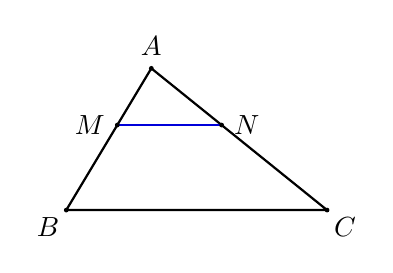
\begin{tikzpicture}[scale=0.72, >=stealth, line join=round, line cap=round]
  \coordinate (B) at (0, 0);
  \coordinate (C) at (4.6, 0);
  \coordinate (A) at (1.5, 2.5);
  \coordinate (M) at (0.9, 1.5);
  \coordinate (N) at (2.74, 1.5);
  \draw[thick] (A) -- (B) -- (C) -- cycle;
  \draw[thick, blue!85!black] (M) -- (N);
  \fill (A) circle (1.2pt) node[above=1pt] {$A$};
  \fill (B) circle (1.2pt) node[below left=-1pt] {$B$};
  \fill (C) circle (1.2pt) node[below right=-1pt] {$C$};
  \fill (M) circle (1.2pt) node[left=1pt] {$M$};
  \fill (N) circle (1.2pt) node[right=1pt] {$N$};
\end{tikzpicture}
\end{minipage}\par
\vspace{0.4mm}
\noindent\textit{Bài giải:}\dongkeHaiCot{11}
\\ \hline
\end{tabularx}

\vspace{1.4mm}

\noindent
\begin{tabularx}{\linewidth}{|X|}
\hline
\vspace{0.5mm}
\textbf{Câu 14 (0,5 điểm).} Tìm giá trị lớn nhất của biểu thức $R = -x^2 + 10x + 2002$.\par
\vspace{0.4mm}
\noindent\textit{Bài giải:}\dongkeHaiCot{7}
\\ \hline
\end{tabularx}

\newpage
% =============================================================================
% ========================= TOAN 8 TUAN 10 BUOI 02 - MA DE 104 =================
% ========================= TRANG 1/2 ==========================================
% =============================================================================
\noindent
\begin{tabularx}{\linewidth}{|X|c|}
\hline
\textbf{PHIẾU KIỂM TRA ĐỊNH KỲ TOÁN 8 - TUẦN 10 - BUỔI 2} & \textbf{Mã đề: 104 - Trang 1/2} \\
\hline
\end{tabularx}

\vspace{1.2mm}

\noindent
\begin{tabularx}{\linewidth}{|p{3.2cm}|X|}
\hline
\centering\textbf{ĐIỂM SỐ} & \centering\textbf{LỜI NHẬN XÉT CỦA THẦY CÔ} \tabularnewline
\hline
\rule{0pt}{1.8cm} & \tabularnewline
\hline
\end{tabularx}

\vspace{1.4mm}
\noindent\textbf{Câu 1 (0,25 điểm).} Cho $\Delta ABC, M \in AB, N \in AC$ có $\dfrac{AM}{MB} = \dfrac{AN}{NC} = \dfrac{1}{2}$. Khi đó $MN \dots BC$: \shortans{\parallel}\par\vspace{2.0mm}
\noindent\textbf{Câu 2 (0,25 điểm).} $\Delta ABC, MN \parallel BC$. Biết $AM=2, AB=8, BC=16\text{ cm}$. Độ dài $MN$ là: \shortans{4\text{ cm}}\par\vspace{2.0mm}
\noindent\textbf{Câu 3 (0,25 điểm).} Cho $\Delta ABC$ có $DE \parallel BC$. Biết $AD=5, DB=2$. Tỉ số $\dfrac{DE}{BC}$ bằng: \shortans{\frac{5}{7}}\par\vspace{2.0mm}
\noindent\textbf{Câu 4 (0,25 điểm).} Phân tích đa thức $2x^2 - 6x$ thành nhân tử được: \shortans{2x(x - 3)}\par\vspace{2.0mm}
\noindent\textbf{Câu 5 (0,25 điểm).} Phân tích đa thức $x^2 - 64$ thành nhân tử được: \shortans{(x - 8)(x + 8)}\par\vspace{2.0mm}
\noindent\textbf{Câu 6 (0,25 điểm).} Thu gọn biểu thức $x^2 - 12x + 36$ thành bình phương được: \shortans{(x - 6)^2}\par\vspace{2.0mm}
\noindent\textbf{Câu 7 (0,25 điểm).} Bậc của đa thức $S = 2x^4 y^2 - 5x^3 y^3 + 4xy^4 + 1$ là: \shortans{6}\par\vspace{2.0mm}
\noindent\textbf{Câu 8 (0,25 điểm).} Kết quả của phép chia $(35x^7 y^4) : (7x^5 y^2)$ là: \shortans{5x^2 y^2}\par\vspace{2.0mm}
\noindent\textbf{Câu 9 (0,25 điểm).} Đường thẳng song song một cạnh tam giác tạo ra các đoạn thẳng: \shortans{\text{tương ứng tỉ lệ}}\par\vspace{2.0mm}
\noindent\textbf{Câu 10 (0,25 điểm).} Bờ sông có $MN \parallel AB$: $OM=4, MA=12, MN=6\text{ m}$. Tính $AB$: \shortans{24\text{ m}}\par\vspace{2.0mm}
\vspace{0.2mm}
\noindent\textbf{Câu 11 (3,0 điểm). Thực hiện phép tính và phân tích đa thức thành nhân tử:}
\vspace{0.8mm}

\noindent
\begin{tabularx}{\linewidth}{|X|X|}
\hline
\oBaiTap[5]{a) (0,5 điểm)}{$3x(3x^2 - 2x + 4)$} & 
\oBaiTap[5]{b) (0,5 điểm)}{$(x - 2)(x + 6) - (x^2 - 12)$} \\
\hline
\oBaiTap[5]{c) (0,5 điểm)}{$(3x - 1)^2 + (3x + 1)^2$} & 
\oBaiTap[5]{d) (0,5 điểm)}{Phân tích nhân tử: $xy - 2x + 4y - 8$} \\
\hline
\oBaiTap[5]{e) (0,5 điểm)}{Phân tích nhân tử: $x^2 - y^2 + 10x + 25$} & 
\oBaiTap[5]{f) (0,5 điểm)}{Phân tích nhân tử: $x^2 - 7x + 10$} \\
\hline
\end{tabularx}

\newpage
% =============================================================================
% ========================= TOAN 8 TUAN 10 BUOI 02 - MA DE 104 =================
% ========================= TRANG 2/2 ==========================================
% =============================================================================
\noindent
\begin{tabularx}{\linewidth}{|X|c|}
\hline
\textbf{TOÁN 8 - TUẦN 10 - BUỔI 2} & \textbf{Mã đề: 104 - Trang 2/2} \\
\hline
\end{tabularx}

\vspace{1.4mm}

\noindent\textbf{Câu 12 (2,0 điểm). Tìm số thực $x$, biết:}
\vspace{0.8mm}

\noindent
\begin{tabularx}{\linewidth}{|X|X|}
\hline
\oBaiTap[5]{a) (0,5 điểm)}{$5x(x - 3) - 5x^2 = 30$} & 
\oBaiTap[5]{b) (0,5 điểm)}{$x(x - 5) - 4(x - 5) = 0$} \\
\hline
\oBaiTap[5]{c) (0,5 điểm)}{$(x - 5)^2 - 16 = 0$} & 
\oBaiTap[5]{d) (0,5 điểm)}{$(3x - 2)^2 = 64$} \\
\hline
\end{tabularx}

\vspace{1.4mm}

\noindent
\begin{tabularx}{\linewidth}{|X|}
\hline
\vspace{0.5mm}
\begin{minipage}[t]{0.68\linewidth}
\vspace{0pt}
\textbf{Câu 13 (2,0 điểm).} Cho tam giác $ABC$. Trên cạnh $AB$ lấy điểm $M$, trên cạnh $AC$ lấy điểm $N$. Cho biết $AM = 5\text{ cm}, MB = 10\text{ cm}, AN = 6\text{ cm}, NC = 12\text{ cm}$ và $BC = 24\text{ cm}$.\par\vspace{0.4mm}
\textbf{a)} \textbf{(1,0 điểm)} Chứng minh rằng $MN \parallel BC$.\par\vspace{0.4mm}
\textbf{b)} \textbf{(1,0 điểm)} Tính độ dài đoạn thẳng $MN$.
\end{minipage}\hfill
\begin{minipage}[t]{0.30\linewidth}
\vspace{0pt}\centering
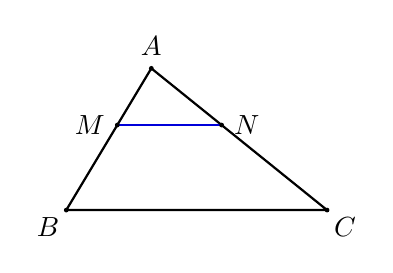
\begin{tikzpicture}[scale=0.72, >=stealth, line join=round, line cap=round]
  \coordinate (B) at (0, 0);
  \coordinate (C) at (4.6, 0);
  \coordinate (A) at (1.5, 2.5);
  \coordinate (M) at (0.9, 1.5);
  \coordinate (N) at (2.74, 1.5);
  \draw[thick] (A) -- (B) -- (C) -- cycle;
  \draw[thick, blue!85!black] (M) -- (N);
  \fill (A) circle (1.2pt) node[above=1pt] {$A$};
  \fill (B) circle (1.2pt) node[below left=-1pt] {$B$};
  \fill (C) circle (1.2pt) node[below right=-1pt] {$C$};
  \fill (M) circle (1.2pt) node[left=1pt] {$M$};
  \fill (N) circle (1.2pt) node[right=1pt] {$N$};
\end{tikzpicture}
\end{minipage}\par
\vspace{0.4mm}
\noindent\textit{Bài giải:}\dongkeHaiCot{11}
\\ \hline
\end{tabularx}

\vspace{1.4mm}

\noindent
\begin{tabularx}{\linewidth}{|X|}
\hline
\vspace{0.5mm}
\textbf{Câu 14 (0,5 điểm).} Tìm giá trị lớn nhất của biểu thức $S = -x^2 + 4x + 2024$.\par
\vspace{0.4mm}
\noindent\textit{Bài giải:}\dongkeHaiCot{7}
\\ \hline
\end{tabularx}
\end{document}
